\documentclass[12pt,a4paper]{article}

\usepackage{float}
\usepackage{cmap}
\usepackage[T1]{fontenc}
\usepackage[utf8x]{inputenc}
\usepackage{amssymb}
\usepackage[danish]{babel}
\usepackage{graphicx}
\usepackage{hyperref}
\usepackage[all]{hypcap}
\hypersetup{
    colorlinks=true,
    linkcolor=blue,
    filecolor=magenta,      
    urlcolor=cyan,
    pdftitle={1g første ugeopgave},
    pdfpagemode=FullScreen,
    }

\urlstyle{same}

\title{PoP - Ugeopgave 1}
\author{Sofie Elisabeth Stone Havn \texttt{<gdx888>}\\ Stine Wittendorff Petersen \texttt{<zcv967>}\\ Sofus Ostrowska Bjørn \texttt{<dxq257>}}
\date{\today}

\begin{document}
\maketitle

\section{Opgave 1g0}

I opgave 1g0 laver vi et lille program ved brug af de ti nævnte scratch blokke. Vi startede med at samle det på papir, hvorefter vi gættede på hvad der vil ske. Vi vil i det følgende beskrive i hvor høj grad programmet opførte sig som forventet. Det simple program kan desuden ses i figur \ref{fig:1}.

\subsection{Proces}
Når spriten klikkes, siger den 'Hello!', også forestiller vi os, at spriten siger 'Meow' indtil den har 'glidet' i x antal sekunder til dens nye koordinater. Dernæst ventes der et sekund, hvorefter den gemmer sig, venter endnu et sekund og ændrer sine koordinater til dens start-koordinater. Til slut viser figuren sig i start positionen, og spillet kan nu startes på ny.
\textit{Play sound Meow until done}, var den eneste blok der ikke opførte sig som forventet. Vi har erfaret at blokken ikke er forbundet til blokken før, men den lyd som den afspillet i stedet... Meget interessant.

\subsection{Forklaring af programmet}
Det viser sig at programmet, som forventet, Siger 'Hello!' i to sekunder når spriten trykkes på, hvorefter den siger 'Meow'. Den bevæger sig hernæst, til koordinaterne x=240, y=140, over fem sekunder. Der ventes nu 1 sekund, så gemmes spriten (Scratch katten), yderligere et sekundt ventes, og spriten (i usynlig tilstand) bliver når rykket til koordinaterne x=0, y=0, og den vises igen. Fra dette stadie kan programmet nu køres igen ved at trykke på spriten.

\begin{figure}[h]
    \centering
    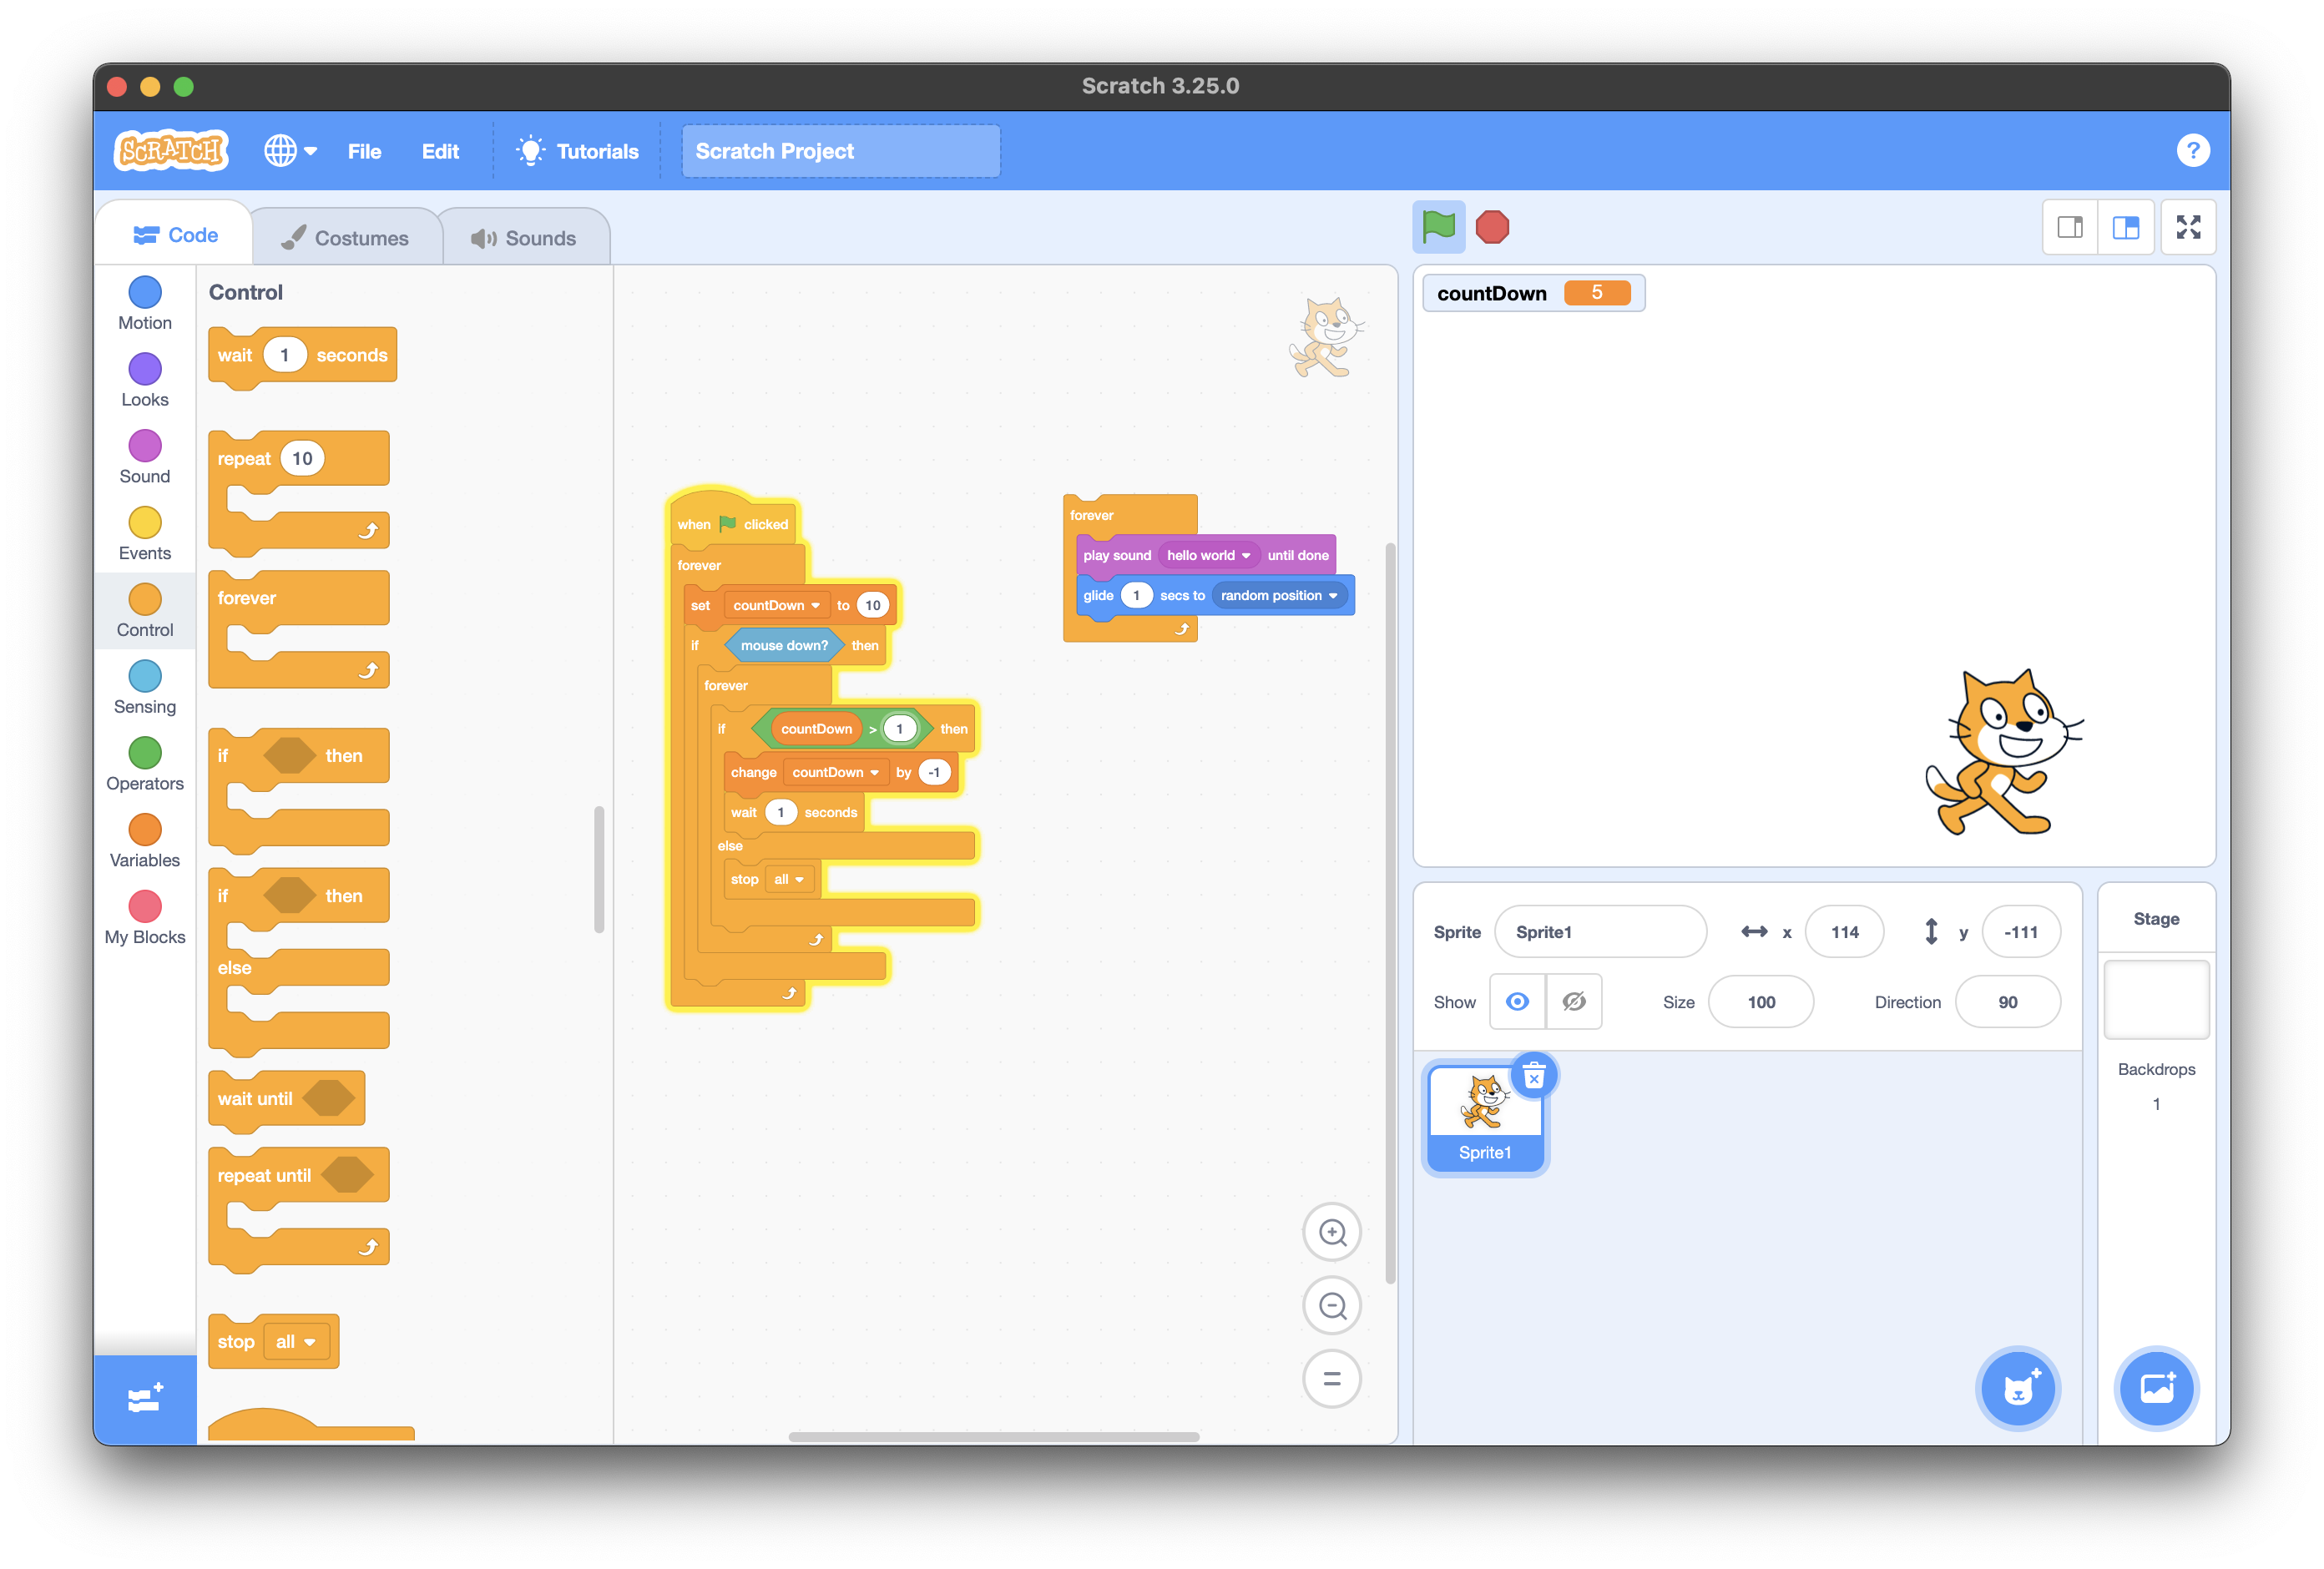
\includegraphics[width=\linewidth]{Evidence.png}
    \caption{Her ses otte ud af de ti blokke i brug}
    \label{fig:1}
\end{figure}
\pagebreak

\section{Opgave 1g1}
Vi er blevet bedt om at lave et Scratch spil som skal indeholde:
\begin{itemize}
    \item 2 til 5 sprites
    \item Omkring et minuts generel spilletid
    \item Inkludere minimum en variable
\end{itemize}
\noindent
Vi startede med at brainstorme hvilket spil vi kunne tænke os at programmere. Vi landte på 'Side-scroller' genren, inspireret af spil som Mario, osv.\\
\linebreak
Dernæst lavede vi en tegning over hvordan spillet skulle se ud; denne har vi dog valgt ikke at inkludere, da tegning ikke var af køn natur.Vi sketchede kort herefter hvordan spillet skulle se ud på papir, men vi valgte kort efter at gå direkte il Scratch, og programmeringen.

\subsection{Proces}
For at lave et sidescroller spil, skal det ligne at baggrunden ‘ruller’ bagved spritten, desuden skal spritten forestille at løbe på jorden hen af skærmen. Dette viste sig at være kompliceret, derfor valgte vi at spritten skulle bevæge sig rundt på den samme baggrund. I stedet for at følge ‘vejen’ kan den ‘flyve’ rundt på hele skærmen, da vi dermed heller ikke behøvedes at tage højde for en realistisk gravitations effekt på figuren. Det betyder at figuren styres med en række simple if-statements, som kan ses i figur \ref{fig:2}. En tidlig version af spillet kan desuden ses i figur \ref{fig:5}\\
\begin{figure}[h]
    \centering
    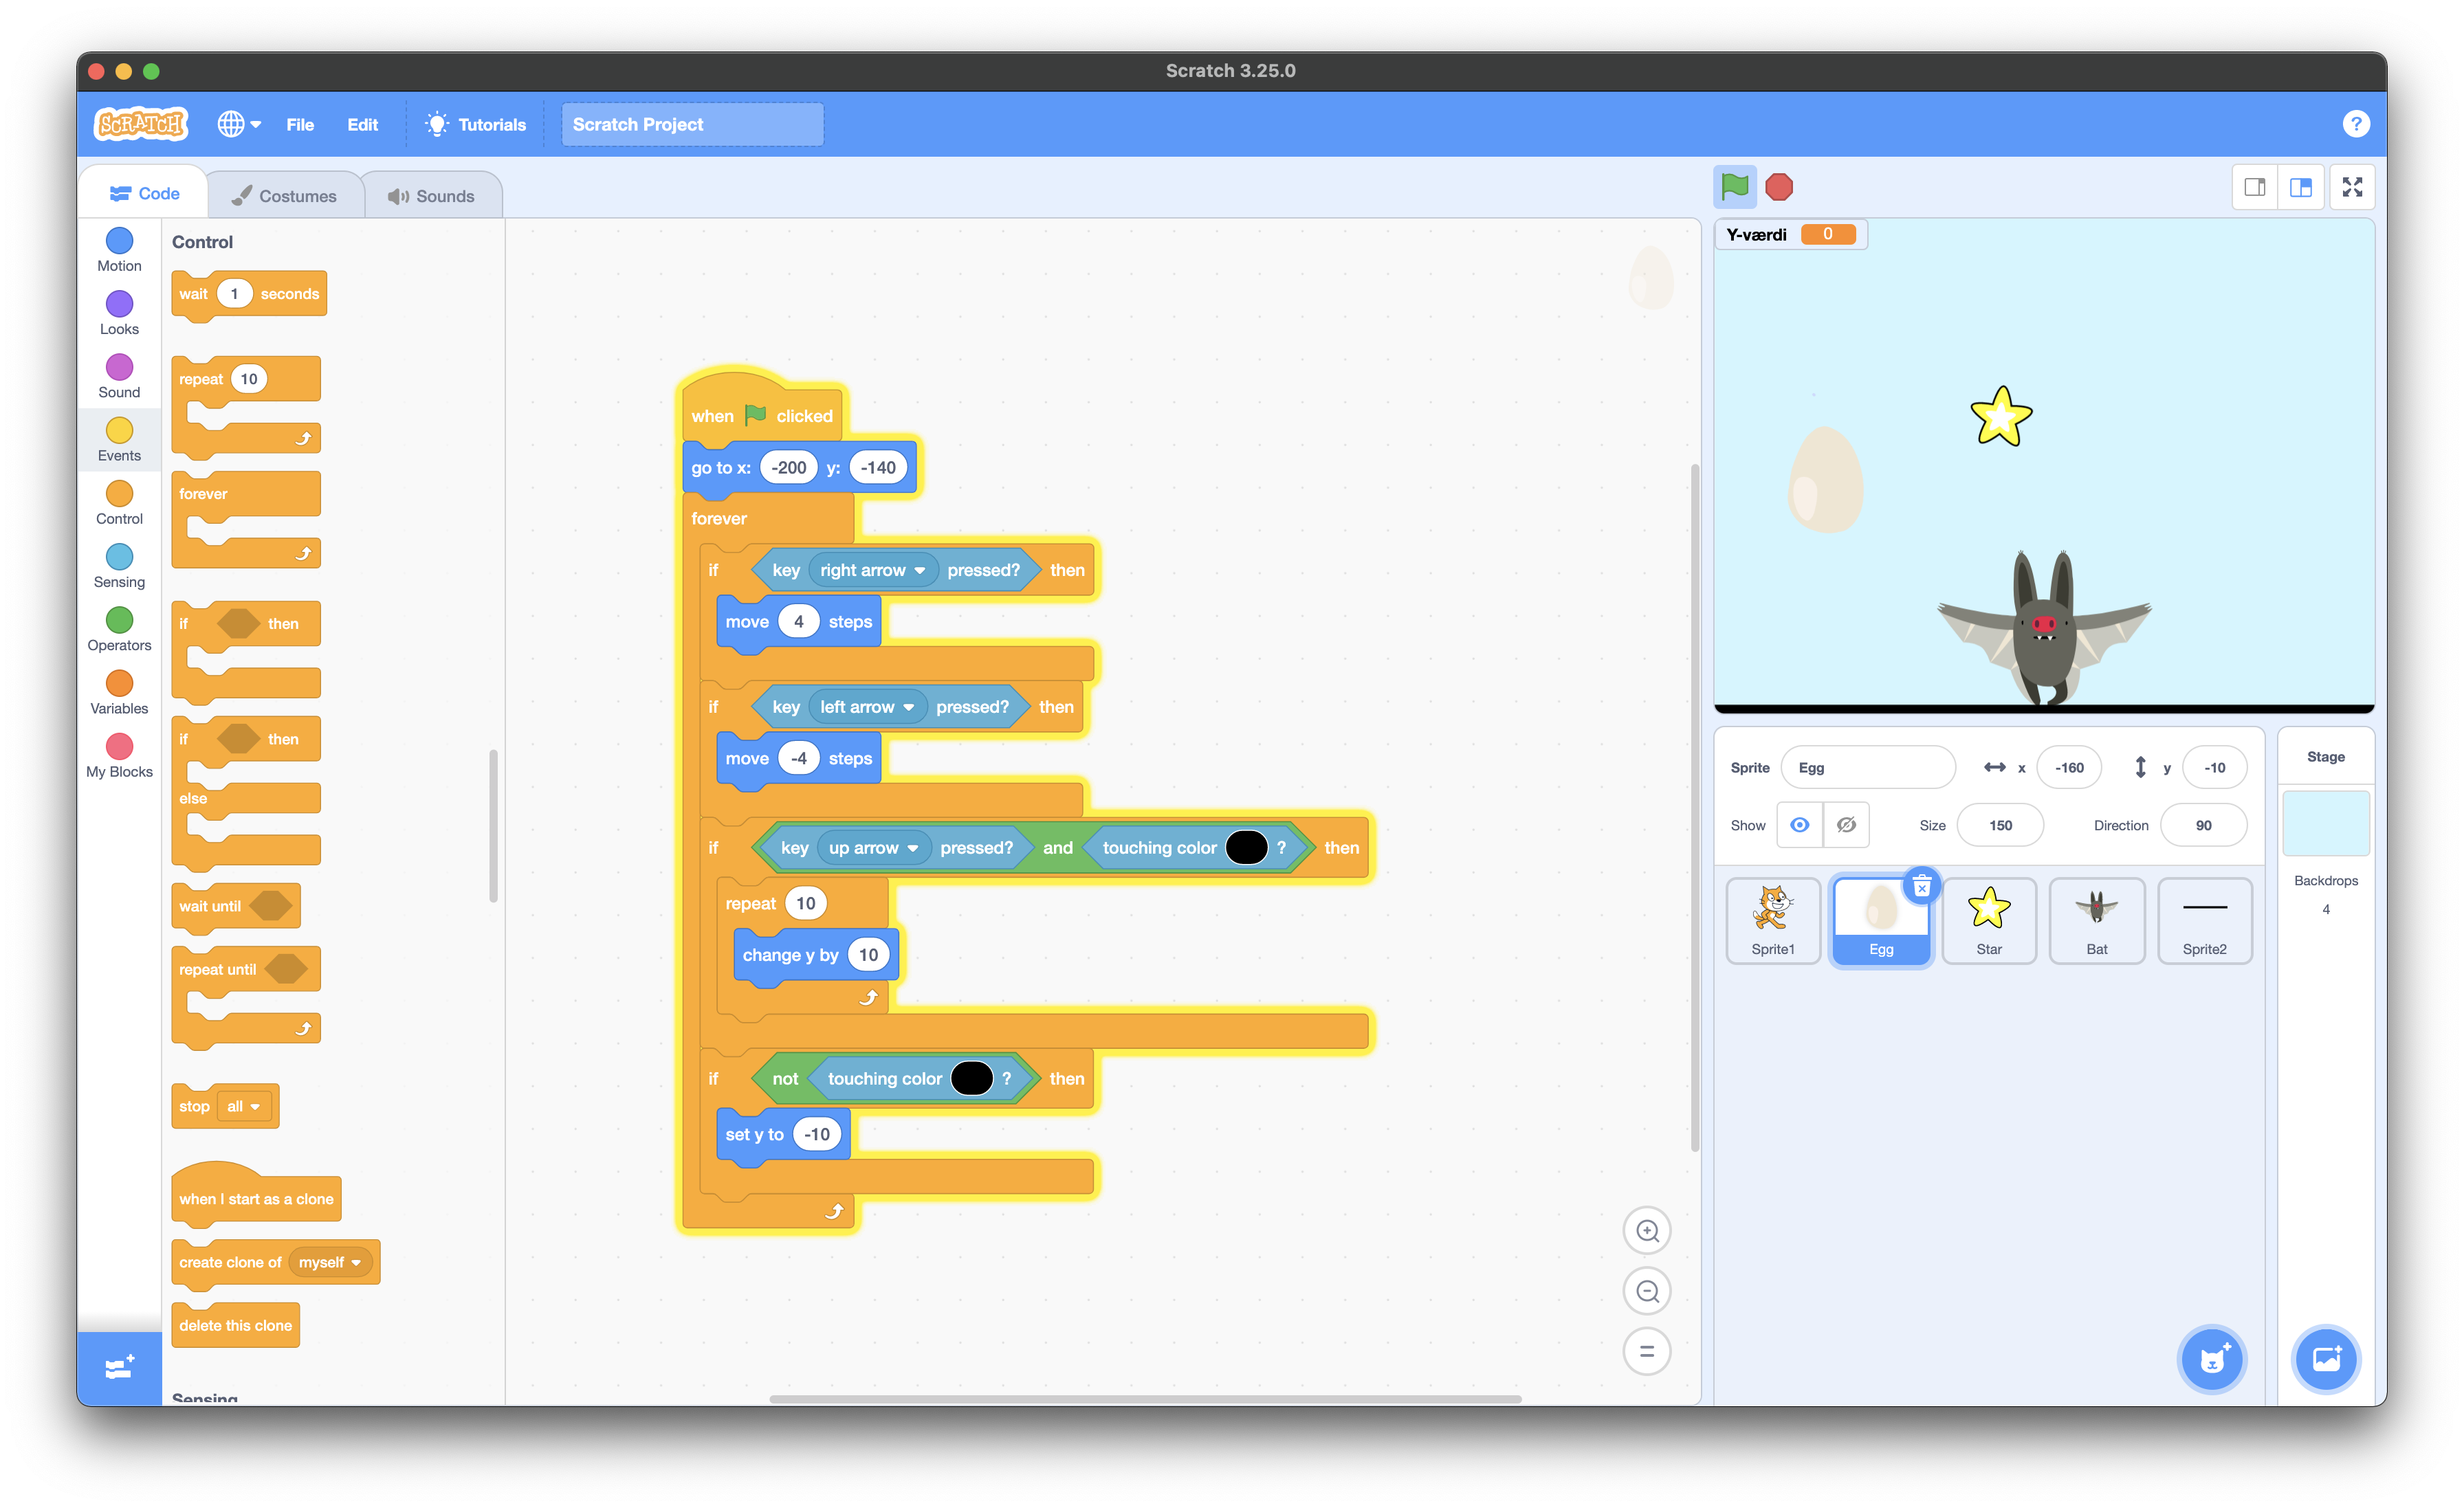
\includegraphics[width=\linewidth]{Tidlig version.png}
    \caption{Her ses en tidlig version af vores spil}
    \label{fig:5}
\end{figure}
\
\linebreak
Vi har også gjort os overvejelser med hensyn til sværhedsgraden af spillet, eksempelvis med forskellige levels.  For at skifte til de forskellige levels har vi benyttet scratches ‘broadcast’ funktion, hvor betingelsen er point-scoren. Et eksempel på dette kan ses i figur \ref{fig:3}
\begin{figure}[h]
    \centering
    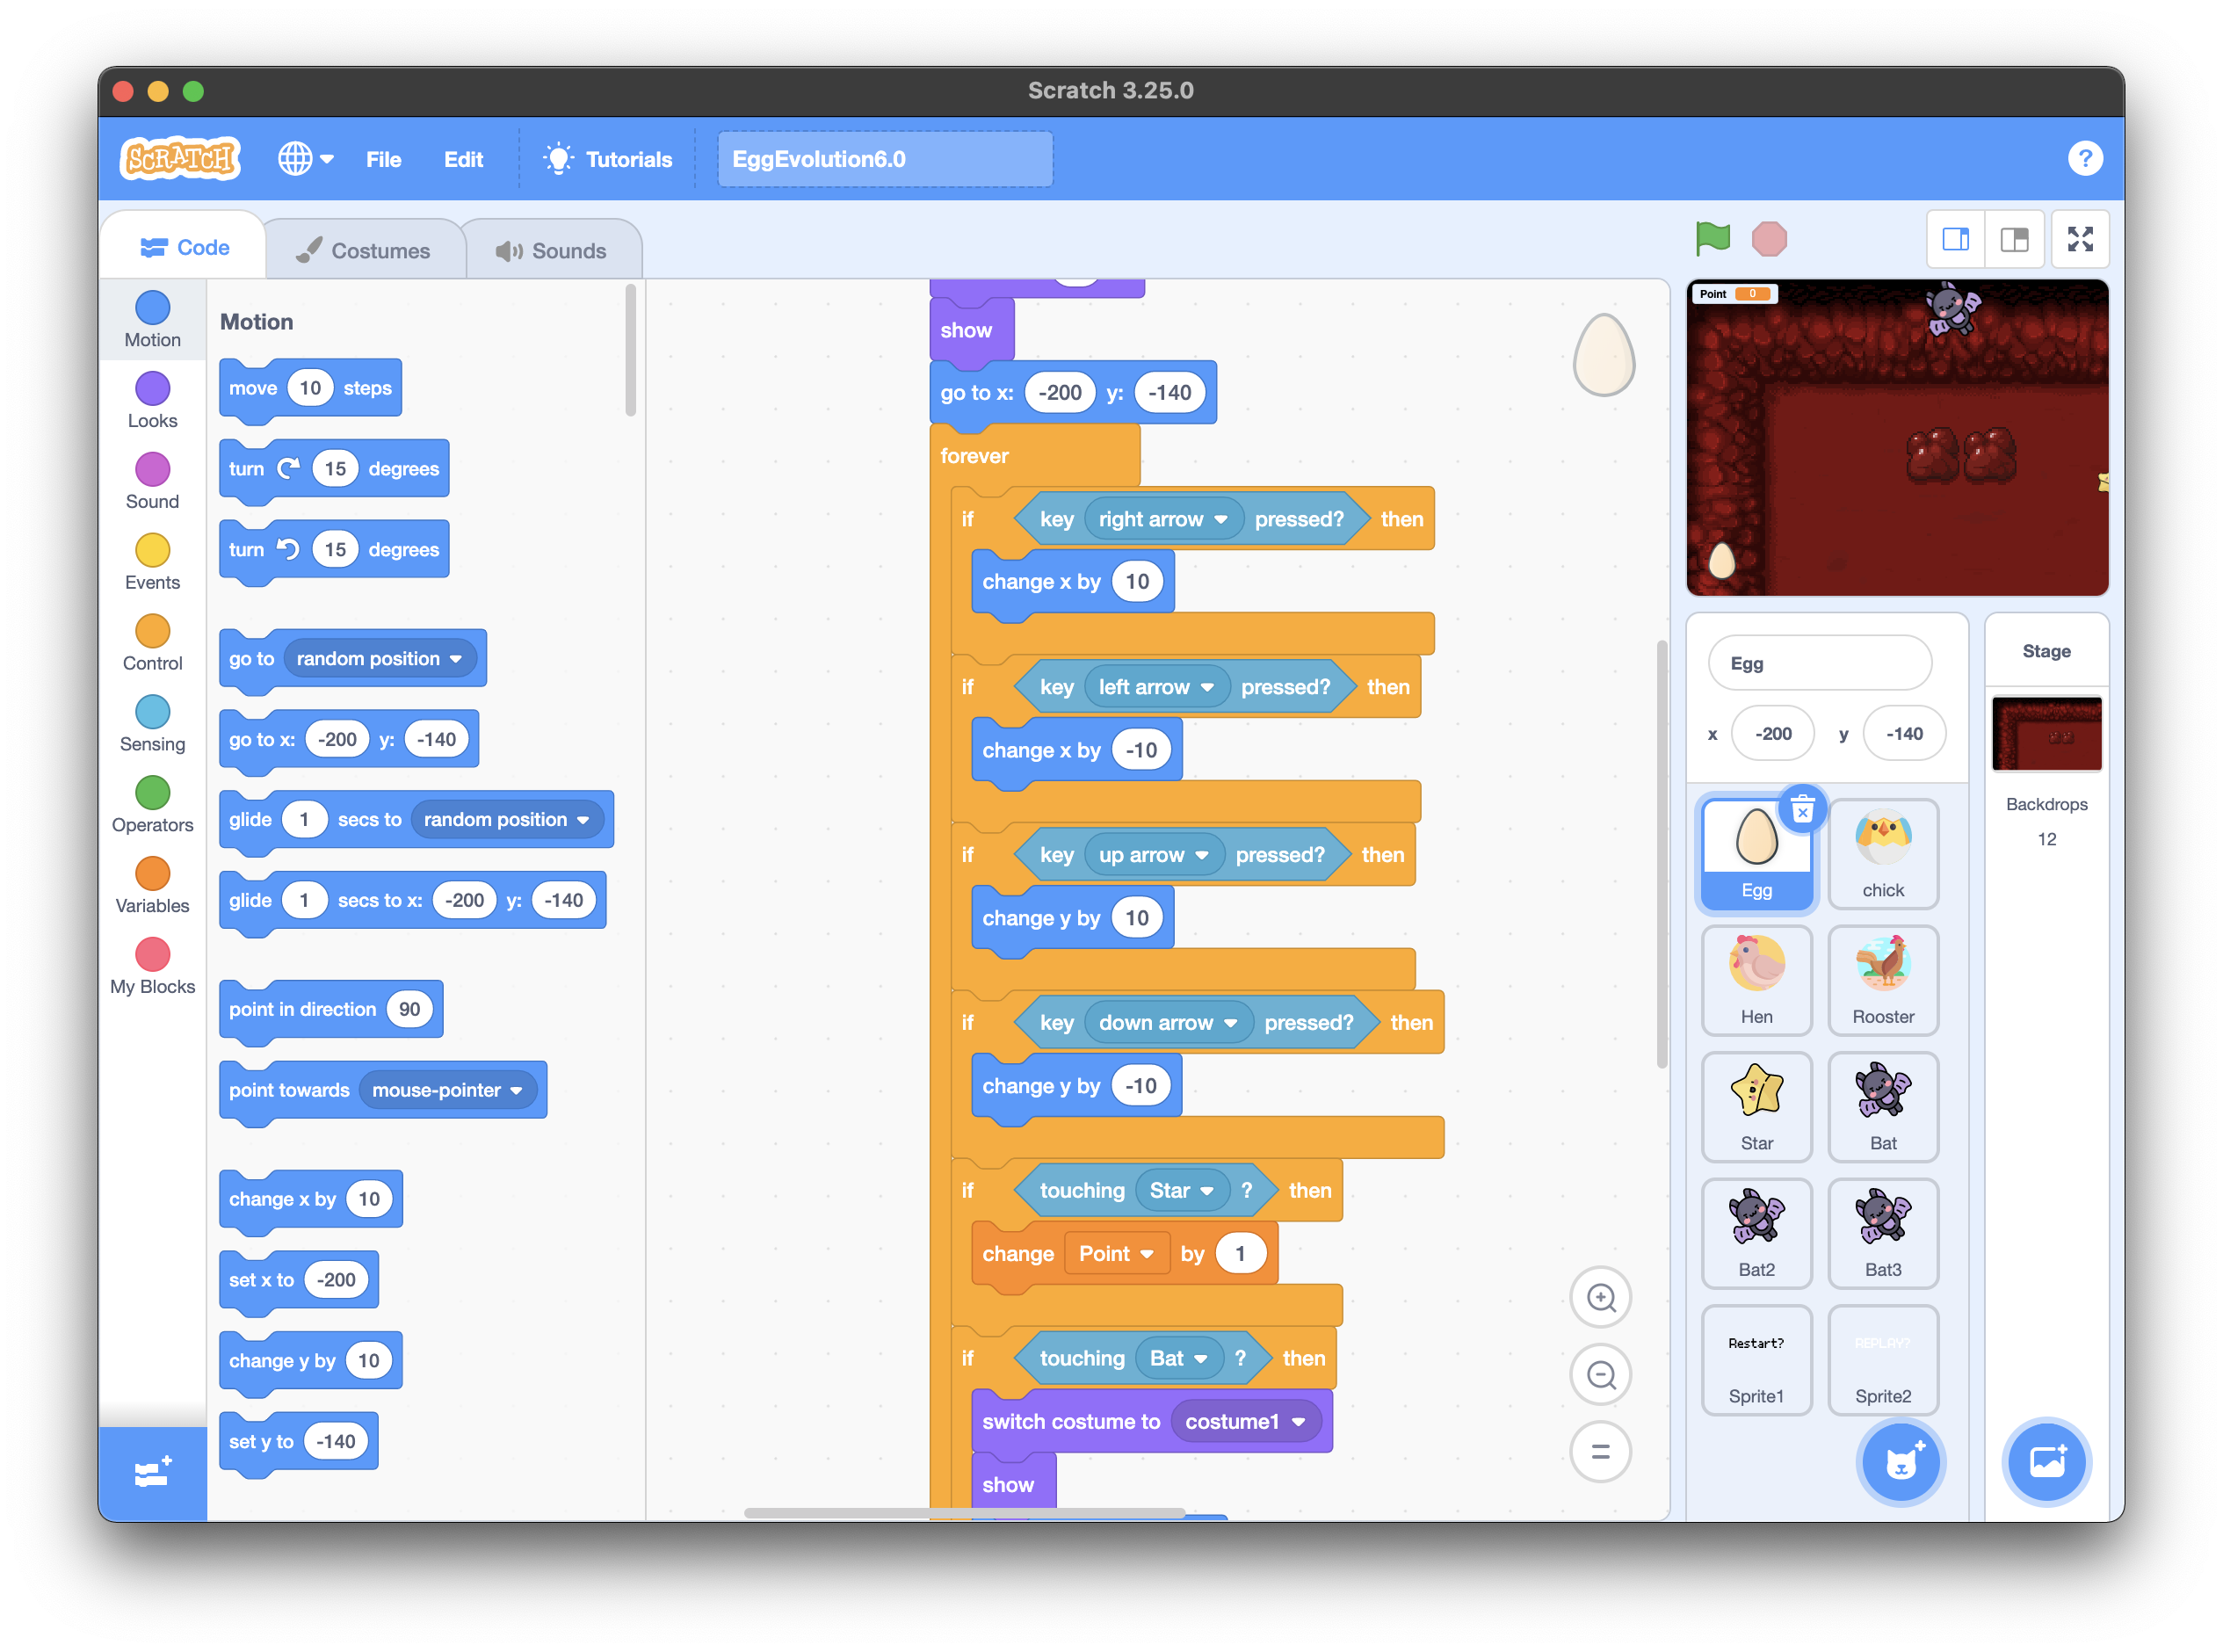
\includegraphics[width=\linewidth]{If-statements.png}
    \caption{Her ses hvordan If-statements bruges til at styre vores sprites}
    \label{fig:2}
\end{figure}\\
\begin{figure}[h]
    \centering
    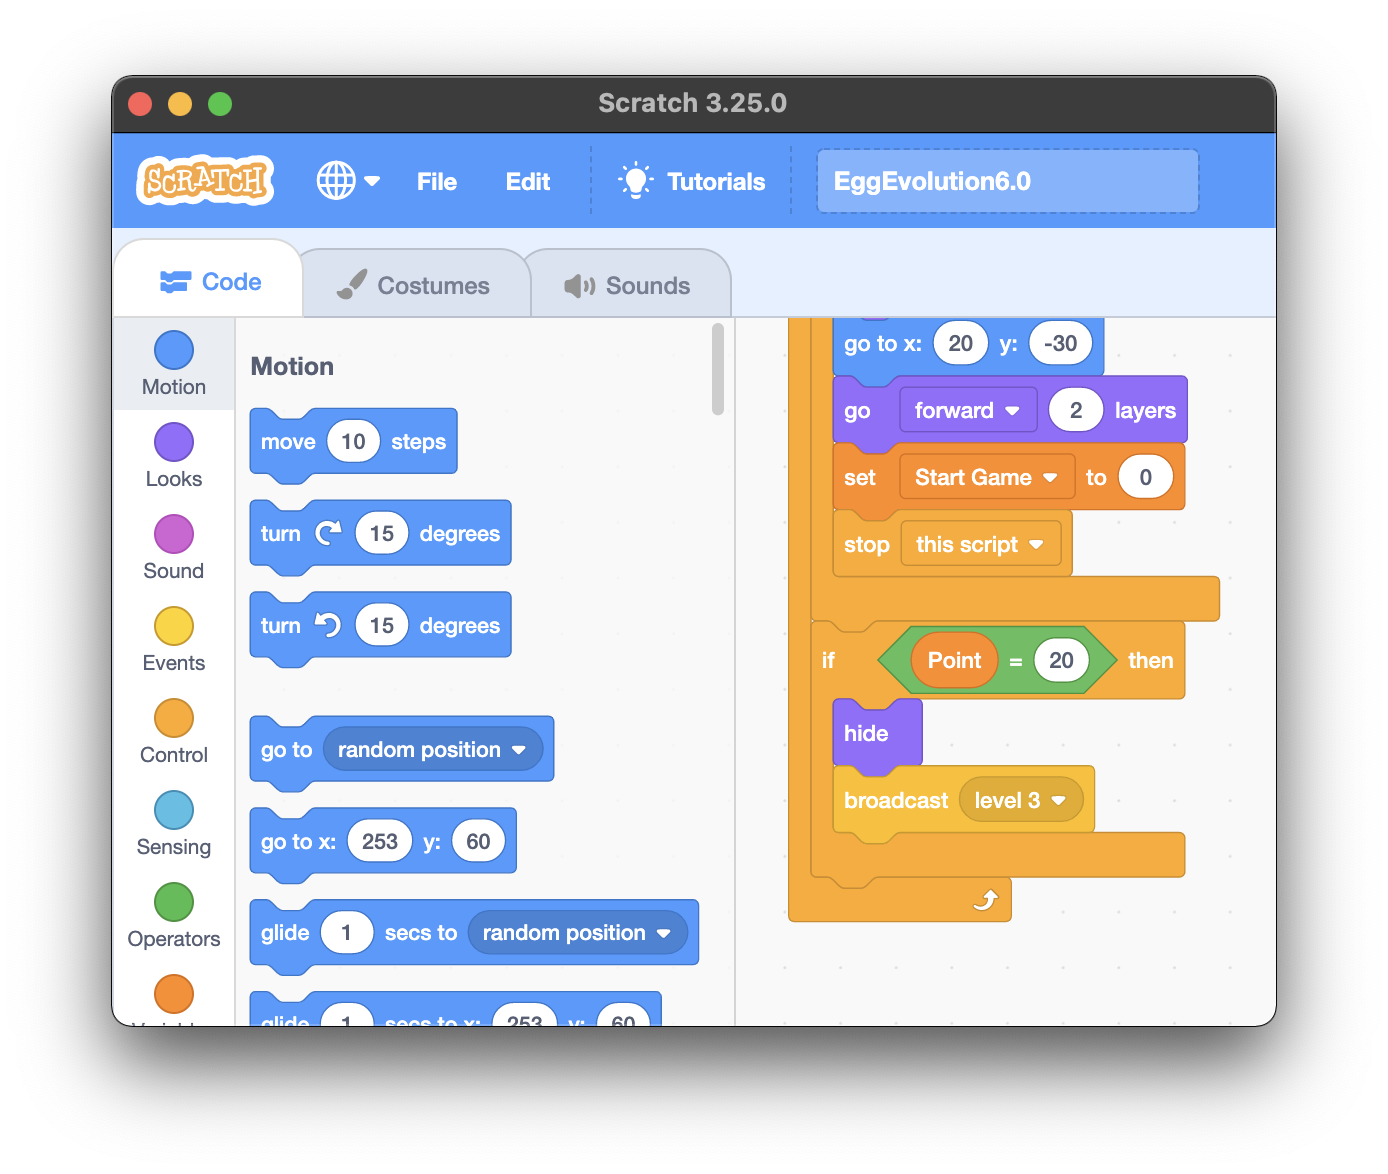
\includegraphics[width=\linewidth]{Broadcast.png}
    \caption{Her ses hvordan Broadcast funktionen afsendes, når et hvis antal point opnåes}
    \label{fig:3}
\end{figure}
\noindent
Vi kom frem til, at der skulle være lidt variation i de forskellige levels, ellers blev det for ensformigt. Vi endte derfor med at sænke hastigheden på flagermusen i level 1 og 2. For at gøre de efterfølgende niveauer sværere, indsatte vi en flagermus mere pr level i 3 og 4. \\
En udfordring vi oplevede, var at vores sprite opstod det samme sted, som flagermusen, når man kom til et nyt level. Dette resulterede i, at man døde med det samme og skulle starte forfra.  
Man kan se, hvordan vi løste det i figur \ref{fig:4}. Til sidst har vi også overvejet spilles æstetik. Spillet er bygget op som en form for evolution, hvor man går fra æg til hane.

\begin{figure}[H]
    \centering
    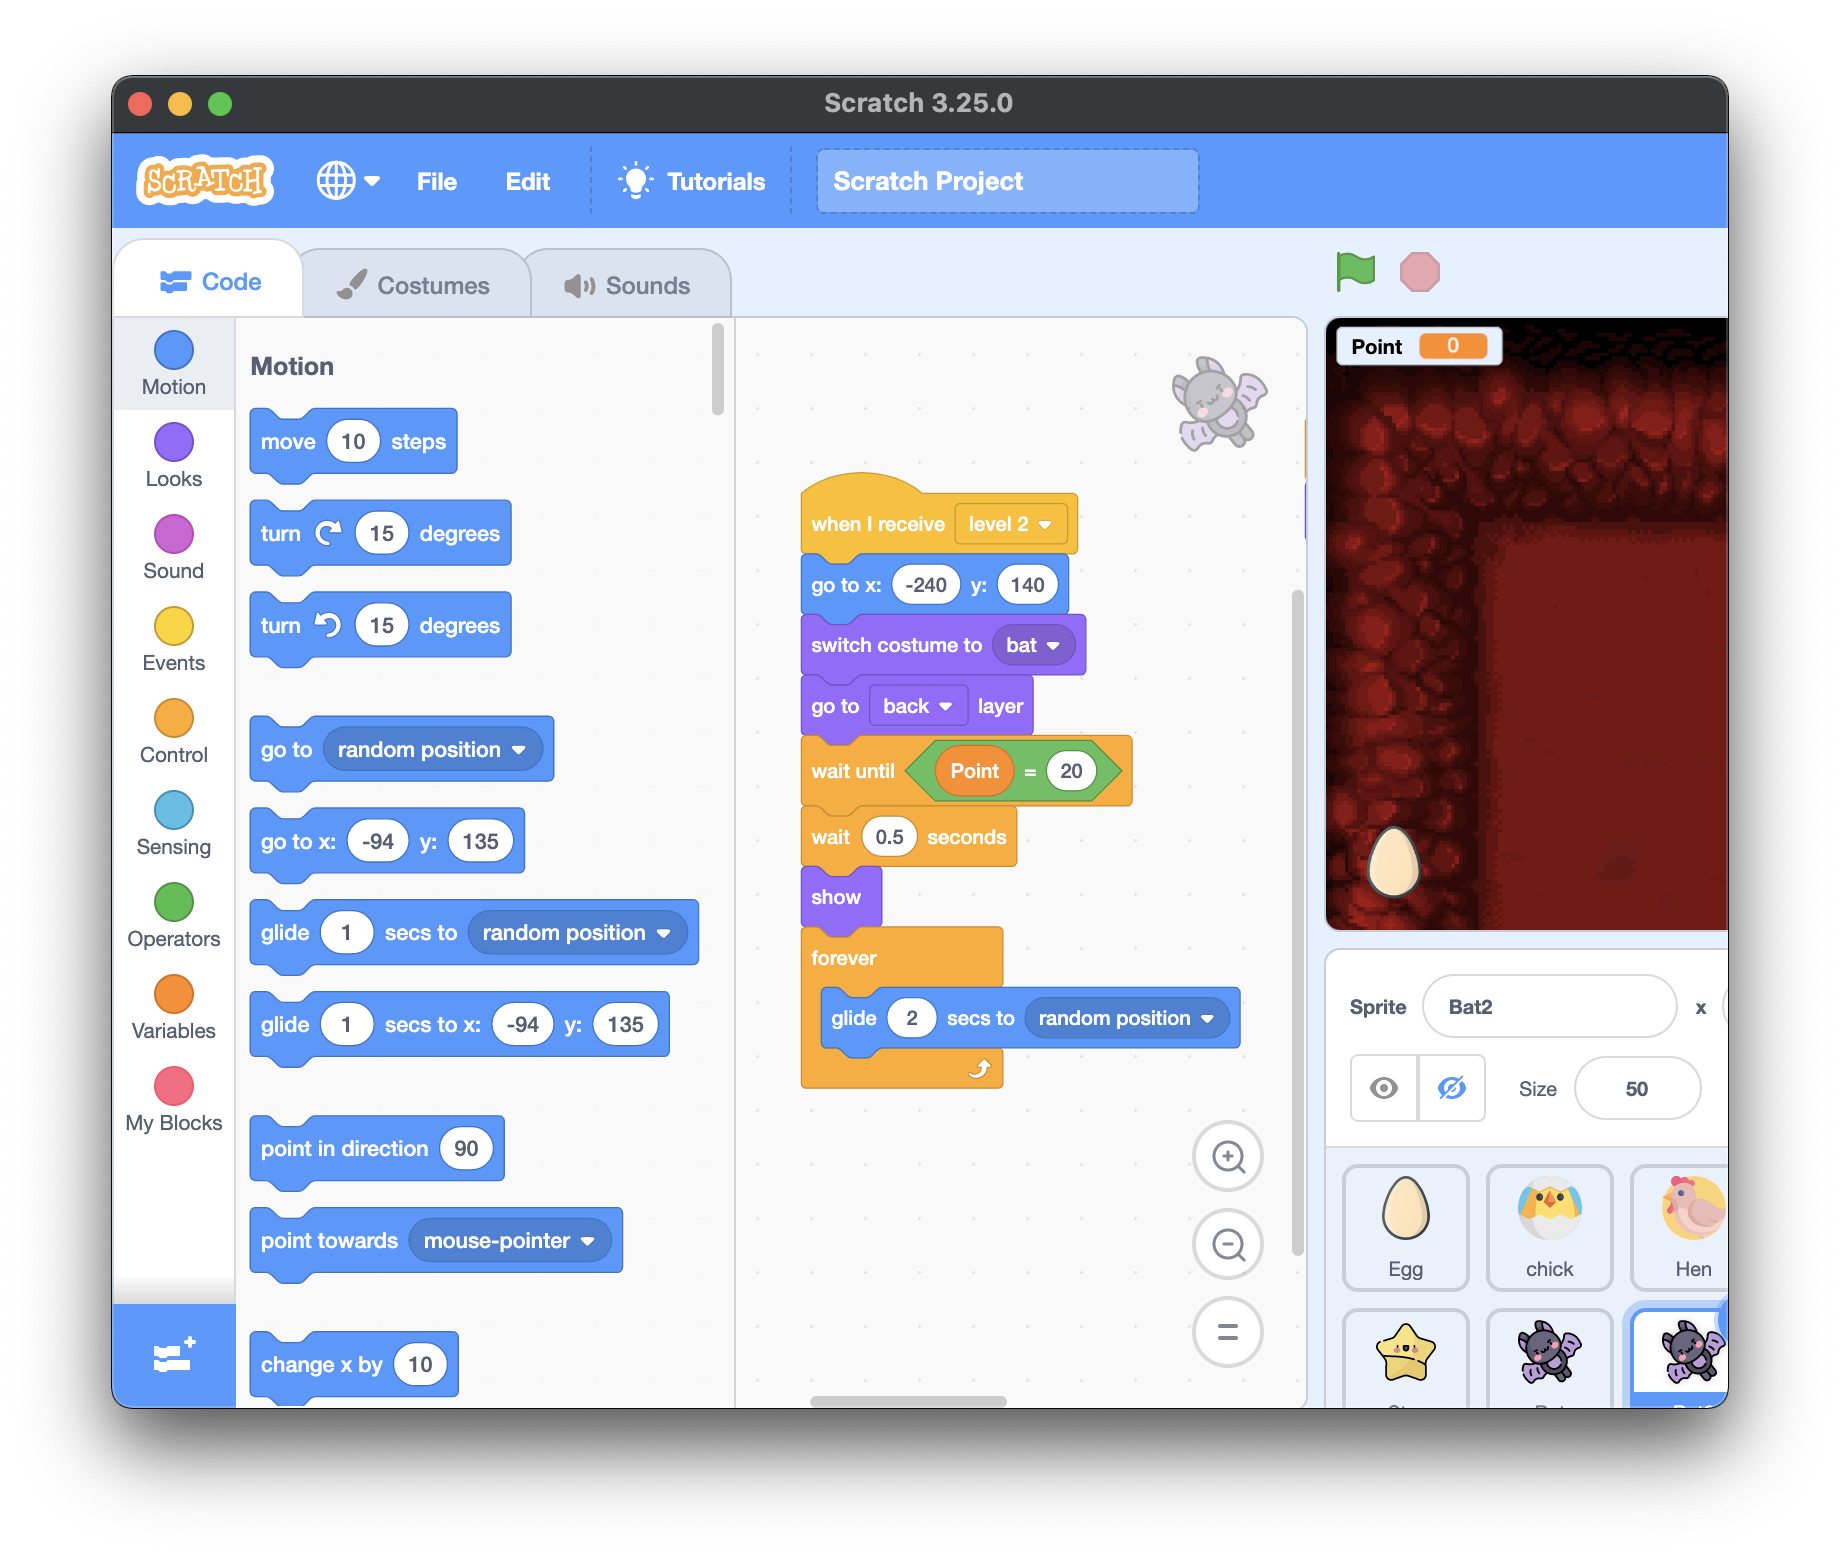
\includegraphics[width=\linewidth]{flagermus.png}
    \caption{Her ses hvordan der undgås at flagermus starter samme sted, som vores sprite}
    \label{fig:4}
\end{figure}
\pagebreak

\subsection{Forklaring af spil}
Vores spil går ud på at man skal samle stjernerne for, at få point og derved stige i level. Målet er at stige til 4. level, uden at støde ind i flagermusene, da de er fysikere. Man starter med 0 point, og kan bevæge sig i alle retninger med piletasterne. Flagermusen 'glider' i level 1, i 3 sekunder i en tilfældig retning (hvilket vil sige relativt langsomt). I level to sættes den til at glide i 2 sekunder i en tilfældig retning. I level 3 støder man på endnu en flagermus der glider over 2 sekunder, og til sidst i level 4, møder man den sidste flagermus der glider over 1 sekund (overraskende hurtigt). Hvis man bliver ramt af en flagermus, bliver man sendt til 'Game Over' skærmen, hvor man har muligheden for trykke på 'Restart' som, uden nogle overraskelser, genstarter spillet. Hvis man når op på 40 point, har man vundet spillet, og har igen mulighed for at trykke på 'REPLAY?' knappen, som giver en mulighed for at spille igen. 

\subsection{Mulige forbedringer}
Her er en liste over de forbedringer vi ville indføre hvis vi havde tilstrækkelig tid og kompetencer:  
\begin{itemize}
\item Nogle gange kommer flagermus nummer 2, ikke frem...
  \item Lade fjender køre til 'edges', i stedet for at de skifter retning efter 'x' sekunder
  \item Skifte sprites'ne til kostumer for at overholde det stillede sprite-interval (2 til 5)
  \begin{itemize}
      \item Dog vil vi argumentere for at grundet flagermusens kopierede natur, at de ikke tæller som en del af de ekstra sprites, selvom vi teknisk set ikke overholder sprite-intervallet. 
      \item En anden ting vi kunne have gjort for, at kunne overholde sprite-intervallet, var at bruge kloner i stedet for at lave en ny sprite. 
      \item Det kan ske at stjernen suser rundt på billedet, når man dør og 'game over' skærmen er der. 
      \item Det er svært at trykke på 'return' eller 'replay', da man skal ramme teksten på en helt speciel måde.
  \end{itemize}
  \item En custom pointtæller
  \item En startskærm (for at undgå at skulle bruge det grønne flag)
  \item Flere levels og større sværhedsgrad
  \item Multiplayer
\end{itemize}


\subsection{Henvisninger}

Vi har brugt nogle elementer fra rundt omkring på nettet. Dette inkludere vores sprites' SVG filer, vores backdrops, og vores musik. Her er en kildehenvisning til hvor vi har fundet det.

\begin{itemize}
    \item SVG iconerne for: Ægget, kyllingen, hønen, hanen, og flagermusen, er lavet af \href{https://www.freepik.com}{Freepik} for \href{www.flaticon.com}{Flaticon} 
    \item \href{https://steamcommunity.com/sharedfiles/filedetails/?l=danish&id=346887557}{Baggrund 1} 
    \item Baggrund 2: Photo by Emiel Maters on \href{https://unsplash.com/photos/2prWrSjtIJg?utm_source=unsplash&utm_medium=referral&utm_content=creditShareLink}{Unsplash} 
    \item Baggrund 3: PPhoto by Michael Jaqua on \href{https://unsplash.com/photos/xYgQYKhfUvo?utm_source=unsplash&utm_medium=referral&utm_content=creditShareLink}{Unsplash} 
    \item Baggrund 4: Photo by Zoe Schaeffer on \href{https://unsplash.com/photos/xYgQYKhfUvo?utm_source=unsplash&utm_medium=referral&utm_content=creditShareLink}{Unsplash} 
    \item Musik fra '8 Bit Nostalgia' af \href{https://www.fesliyanstudios.com/royalty-free-music/download/8-bit-nostalgia/2289}{David Renda} 
\end{itemize}
Desuden har vi fundet inspiration fra følgende kilder, dog har vi ikke udførligt brugt nogle af disse, da vi skiftede retning tidligt i projektet.

\begin{itemize}
    \item  \href{https://en.scratch-wiki.info/wiki/Jumping}{Scratch's egen guide}
    \item  \href{https://scratch.mit.edu/projects/635949/editor/}{En andens Scratch Program}
\end{itemize}

\subsection{Link til Scratch program}

    \href{https://scratch.mit.edu/projects/568368631}{Link til vores spil}

\end{document}
